\usepackage{sansmathaccent}
\pdfmapfile{+sansmathaccent.map}	
	\documentclass[11pt]{beamer}

%%%%%%%%%%%%%%% PACKAGES %%%%%%%%%%%%%%%

\usepackage{url}
\usepackage{amssymb}
\usepackage{tabularx}
\usepackage{graphicx}
\usepackage{amsmath}
\usepackage{amsfonts}
\usepackage{amsthm}
\usepackage{amscd}
\usepackage{graphicx}
\graphicspath{ {./images/} }

%%%%%%%%%%%%%%% BEAMER THEME %%%%%%%%%%%%%%%

\usetheme{Warsaw}

%%%%%%%%%%%%%%% TITLE/AUTHOR INFORMATION %%%%%%%%%%%%%%%

\title{	Cryptography and the World of the Mystery }
\author{Ismail Kably \& Duc Phan}
\date{\today}

%%%%%%%%%%%%%%% PREAMBLE %%%%%%%%%%%%%%%

\newcommand{\Z}{\mathbb{Z}}
\newcommand{\Q}{\mathbb{Q}}
\newcommand{\R}{\mathbb{R}}
\newcommand{\C}{\mathbb{C}}
\newcommand{\norm}[1]{\left\lvert#1\right\rvert}    % Norm

%%%%%%%%%%%%%%% BEGIN DOCUMENT %%%%%%%%%%%%%%%

\begin{document}

\begin{frame}
	
	\titlepage
	
\end{frame}

\begin{frame}\frametitle{Table of Contents}
	
	\tableofcontents
	
\end{frame}

\section{Introduction}

\begin{frame}\frametitle{What we are going to do?}
	
\center Let's explore the world of encryption!
\center 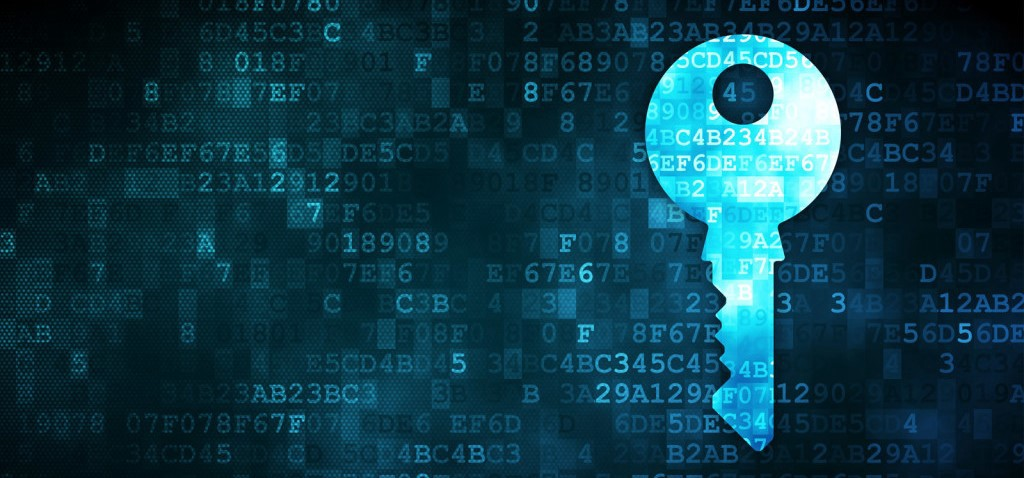
\includegraphics[scale=0.2]{encryption.png}
\end{frame}

\section{What is Cryptography}
\begin{frame}\frametitle{What is cryptography?}
	\begin{enumerate}[a.]
	\item Cryptography or cryptology is the practice and study of techniques for secure communication in the presence of third parties called adversaries.
	\item More generally, cryptography is about constructing and analyzing protocols that prevent third parties or the public from reading private messages.
	\end{enumerate}
\end{frame}

\section{How does Linear Algebra and Encryption connected?}

\begin{frame}\frametitle{The link between Linear Algebra and Encryption}

Because many types of encryption Matrix use the Math behind matrices to encrypt, Linear Algebra is required for Encryption and Decryption!

\end{frame}

\begin{frame}\frametitle{Is it complicated?}
\begin{enumerate}[a.]
	\item The idea behind encryption is not hard to understand at all! 
	\item Cipher matrix can be as simple as a 3x3 matrix composed of random 	integers that represent the characters in the plain-text.
\end{enumerate}

\end{frame}

\section{The fundamental example of Encryption}
\begin{frame}\frametitle{A simple encryption method}
\center Let's take a look at a simple encryption type :D
\center Say, I want to encrypt the word "MATH"
\end{frame}

\begin{frame}\frametitle{The general Idea}
\begin{enumerate}[1]
	\item Convert a plain-text to a matrix
	\item Encrypt the matrix
	\item Decrypt the encrypted matrix
\end{enumerate}
\end{frame}

\begin{frame}\frametitle{Plain-text to Matrix}

Each \textbf{character} in plain-text must be denoted with a \textbf{numerical value} and placed into a matrix.
\center 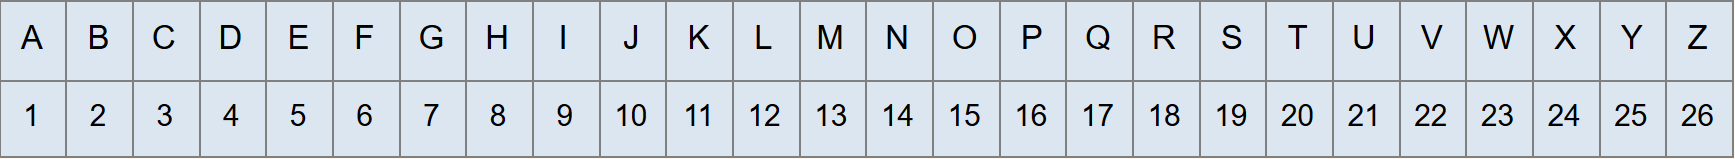
\includegraphics[scale=0.275]{numerical.png}
\end{frame}

\begin{frame}\frametitle{Plain-text to Matrix}

\small The \textbf{numerical values} are then separated into \textbf{vectors}, such that:\\
\begin{enumerate}[a]

\item \scriptsize The number of \textbf{rows} of each \textbf{vector} is equivalent to the numbers of rows of the \textbf{cipher matrix}. \par
\item \textbf{Values} are placed \textbf{one at a time}, \textbf{going down} a row for each value.
\item Vectors are filled \textbf{one to another}.
\item The remaining \textbf{empty entries} in the \textbf{last vector} is filled with \textbf{space}.
\center 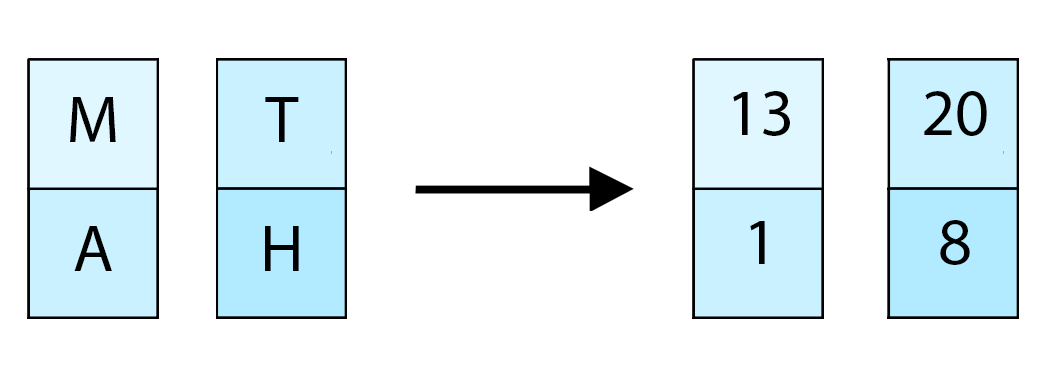
\includegraphics[scale=0.2]{math_1.png}

\end{enumerate}
\end{frame}

\begin{frame}\frametitle{Plain-text to Matrix}

The vectors are then \textbf{augmented} to form a \textbf{plain-text matrix}.
\center 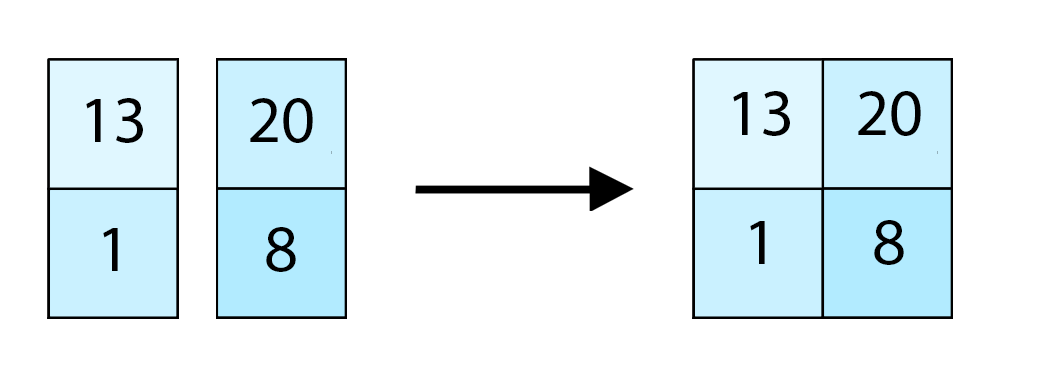
\includegraphics[scale=0.2]{MATH.png}

\end{frame}

\begin{frame}\frametitle{Encrypting the matrix}

The plain-text matrix is then \textbf{multiplied} by another \textbf{cipher-matrix} to create the \textbf{encrypted matrix}.
\center 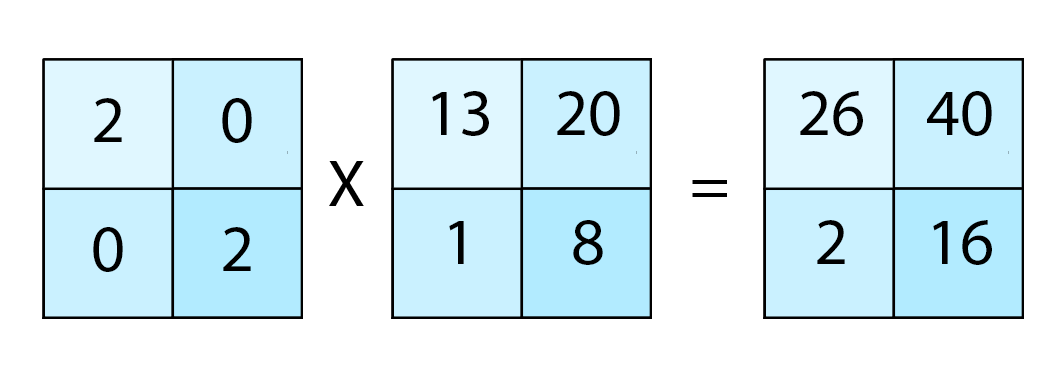
\includegraphics[scale=0.2]{multiply_1.png}

\end{frame}

\begin{frame}\frametitle{Decrypting the matrix}
	\center Let's take a look at this
	\begin{align*}
		& &&C \times P &&&= E\\
		&\iff &&C^{-1} \times C \times P &&&= C^{-1} \times E\\
		&\iff &&P &&&= C^{-1} \times E\\
	\end{align*}
\end{frame}

\begin{frame}\frametitle{Decrypting the matrix}

First, we need to find the \textbf{inverse} of the \textbf{cipher-matrix}.\\[10mm]
\center 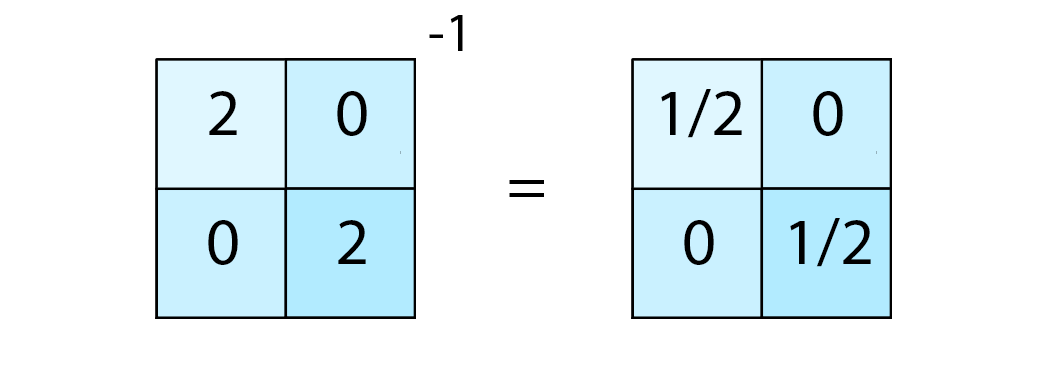
\includegraphics[scale=0.2]{inverse_1.png}
\end{frame}

\begin{frame}\frametitle{Decrypting the matrix}

The \textbf{inverted matrix} is then \textbf{multiplied} with the \textbf{cipher-text matrix}.
The \textbf{product} is the original \textbf{plain-text matrix}.
\center 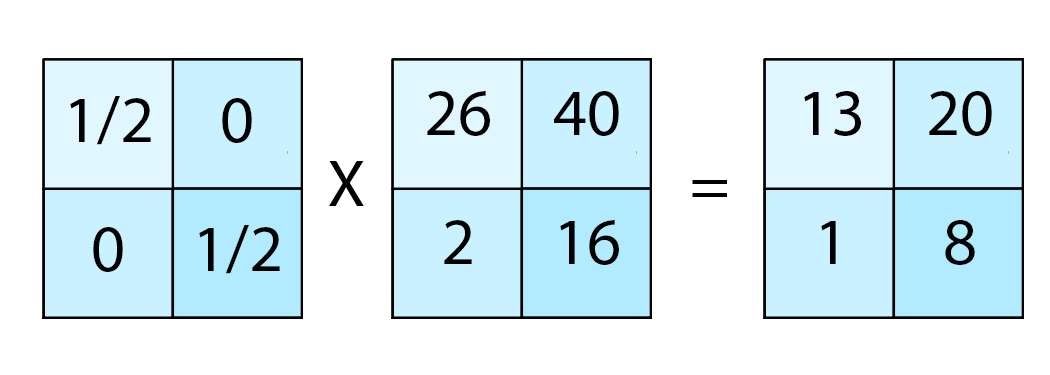
\includegraphics[scale=0.2]{multiply_2.png}
\end{frame}

\begin{frame}\frametitle{Decrypting the matrix}

The \textbf{plain-text} can be found by \textbf{splitting} the \textbf{products} into \textbf{vectors}
\center \includegraphics[scale=0.2]{linear_2.png}

\end{frame}

\begin{frame}\frametitle{Decrypting the matrix}

And then use the \textbf{numerical rules} to convert the \textbf{numbers} back into their \textbf{letter forms}.
\center 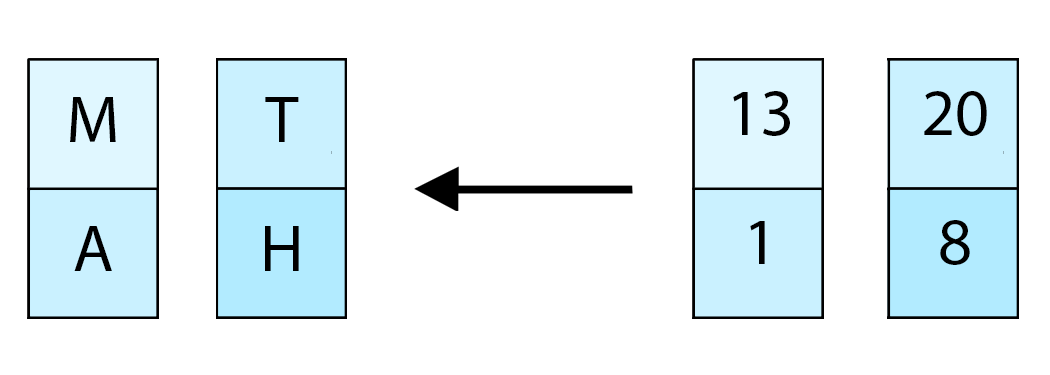
\includegraphics[scale=0.2]{math_2.png}

\end{frame}

\section{AES - Advanced Encryption Standard}
\begin{frame}\frametitle{More advanced encryption}
\center Let's take a look at AES, a more secure encryption type!
\end{frame}

\begin{frame}\frametitle{AES - ...}
	AES - Advanced Encryption Standard - is: 
	\begin{enumerate}[a.]
	\item a symmetric encryption algorithm.
	\item very powerful.
	\item widely used in software and hardware throughout the world! 
	\end{enumerate}
\end{frame}

\begin{frame}\frametitle{The general Process}
	\begin{enumerate}[a.]
	\item AES operates on 4x4 matrix.
	\item Each character in the plain-text is denoted with a corresponding numerical value
	\end{enumerate}
\end{frame}

\begin{frame}\frametitle{An example}
\center Let's take a look at an example to understand the process
\center We'll encrypt and decrypt the plain-text:
\center "Come here I got cash"

\end{frame}

\begin{frame}\frametitle{From text to plain-text matrix}
	Just like in the last example, we use the same rules to convert the text into a matrix. 
	\center 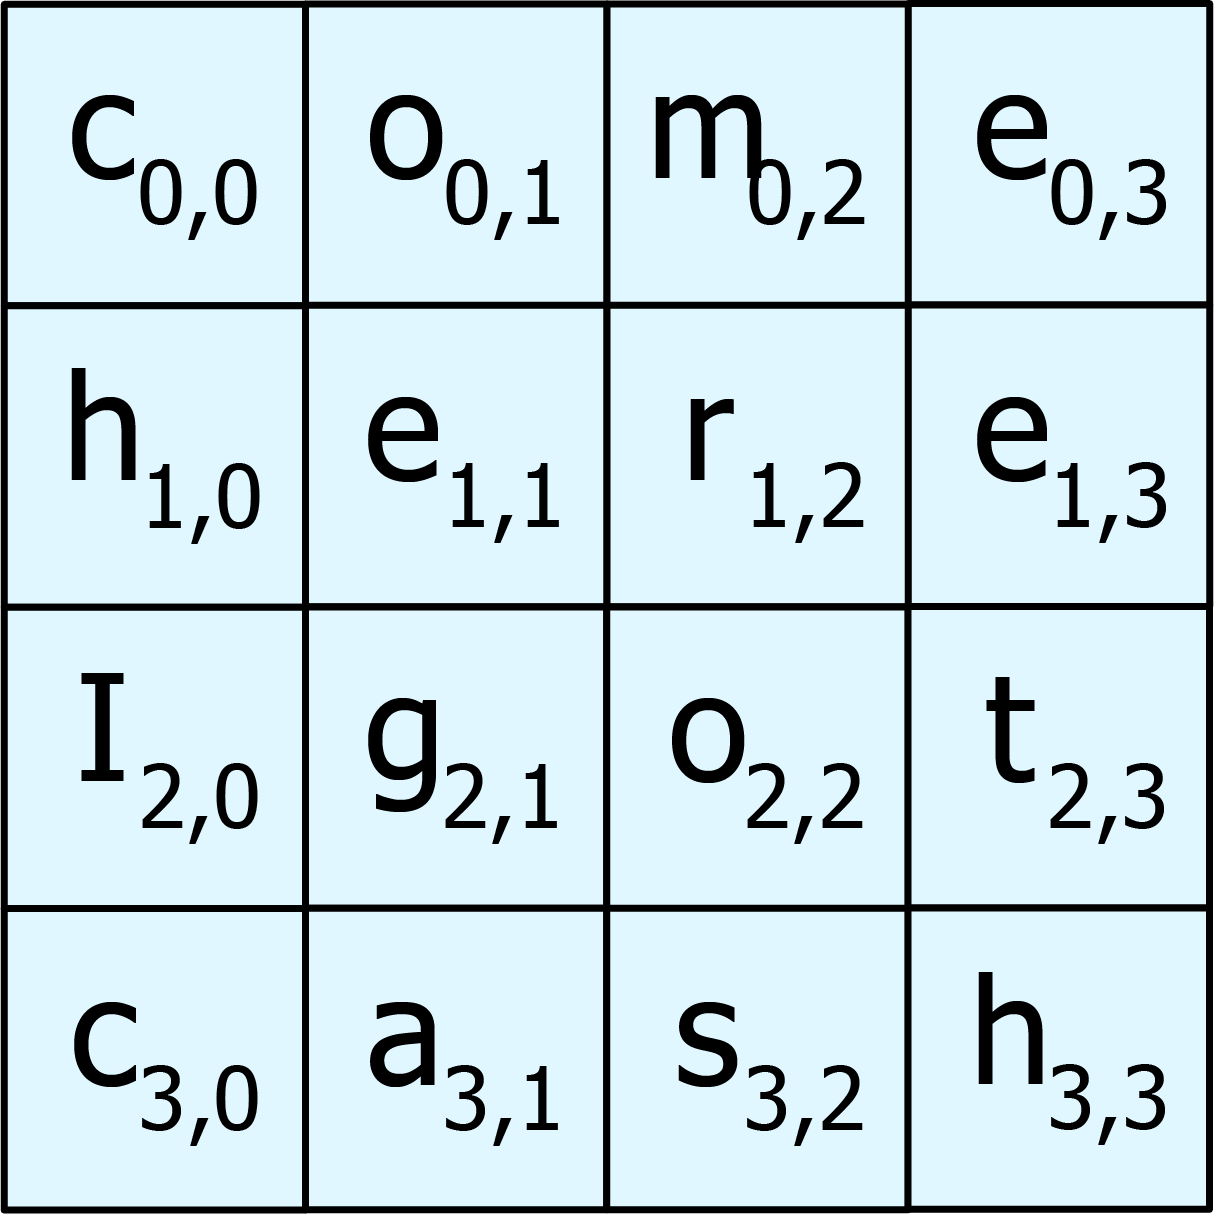
\includegraphics[scale=0.3]{initial_matrix_1.png}

\end{frame}

\begin{frame}\frametitle{Conversion Plain-text to Numerical Matrix}
\footnotesize Then, we convert the plain-text into its corresponding numerical matrix 
\center 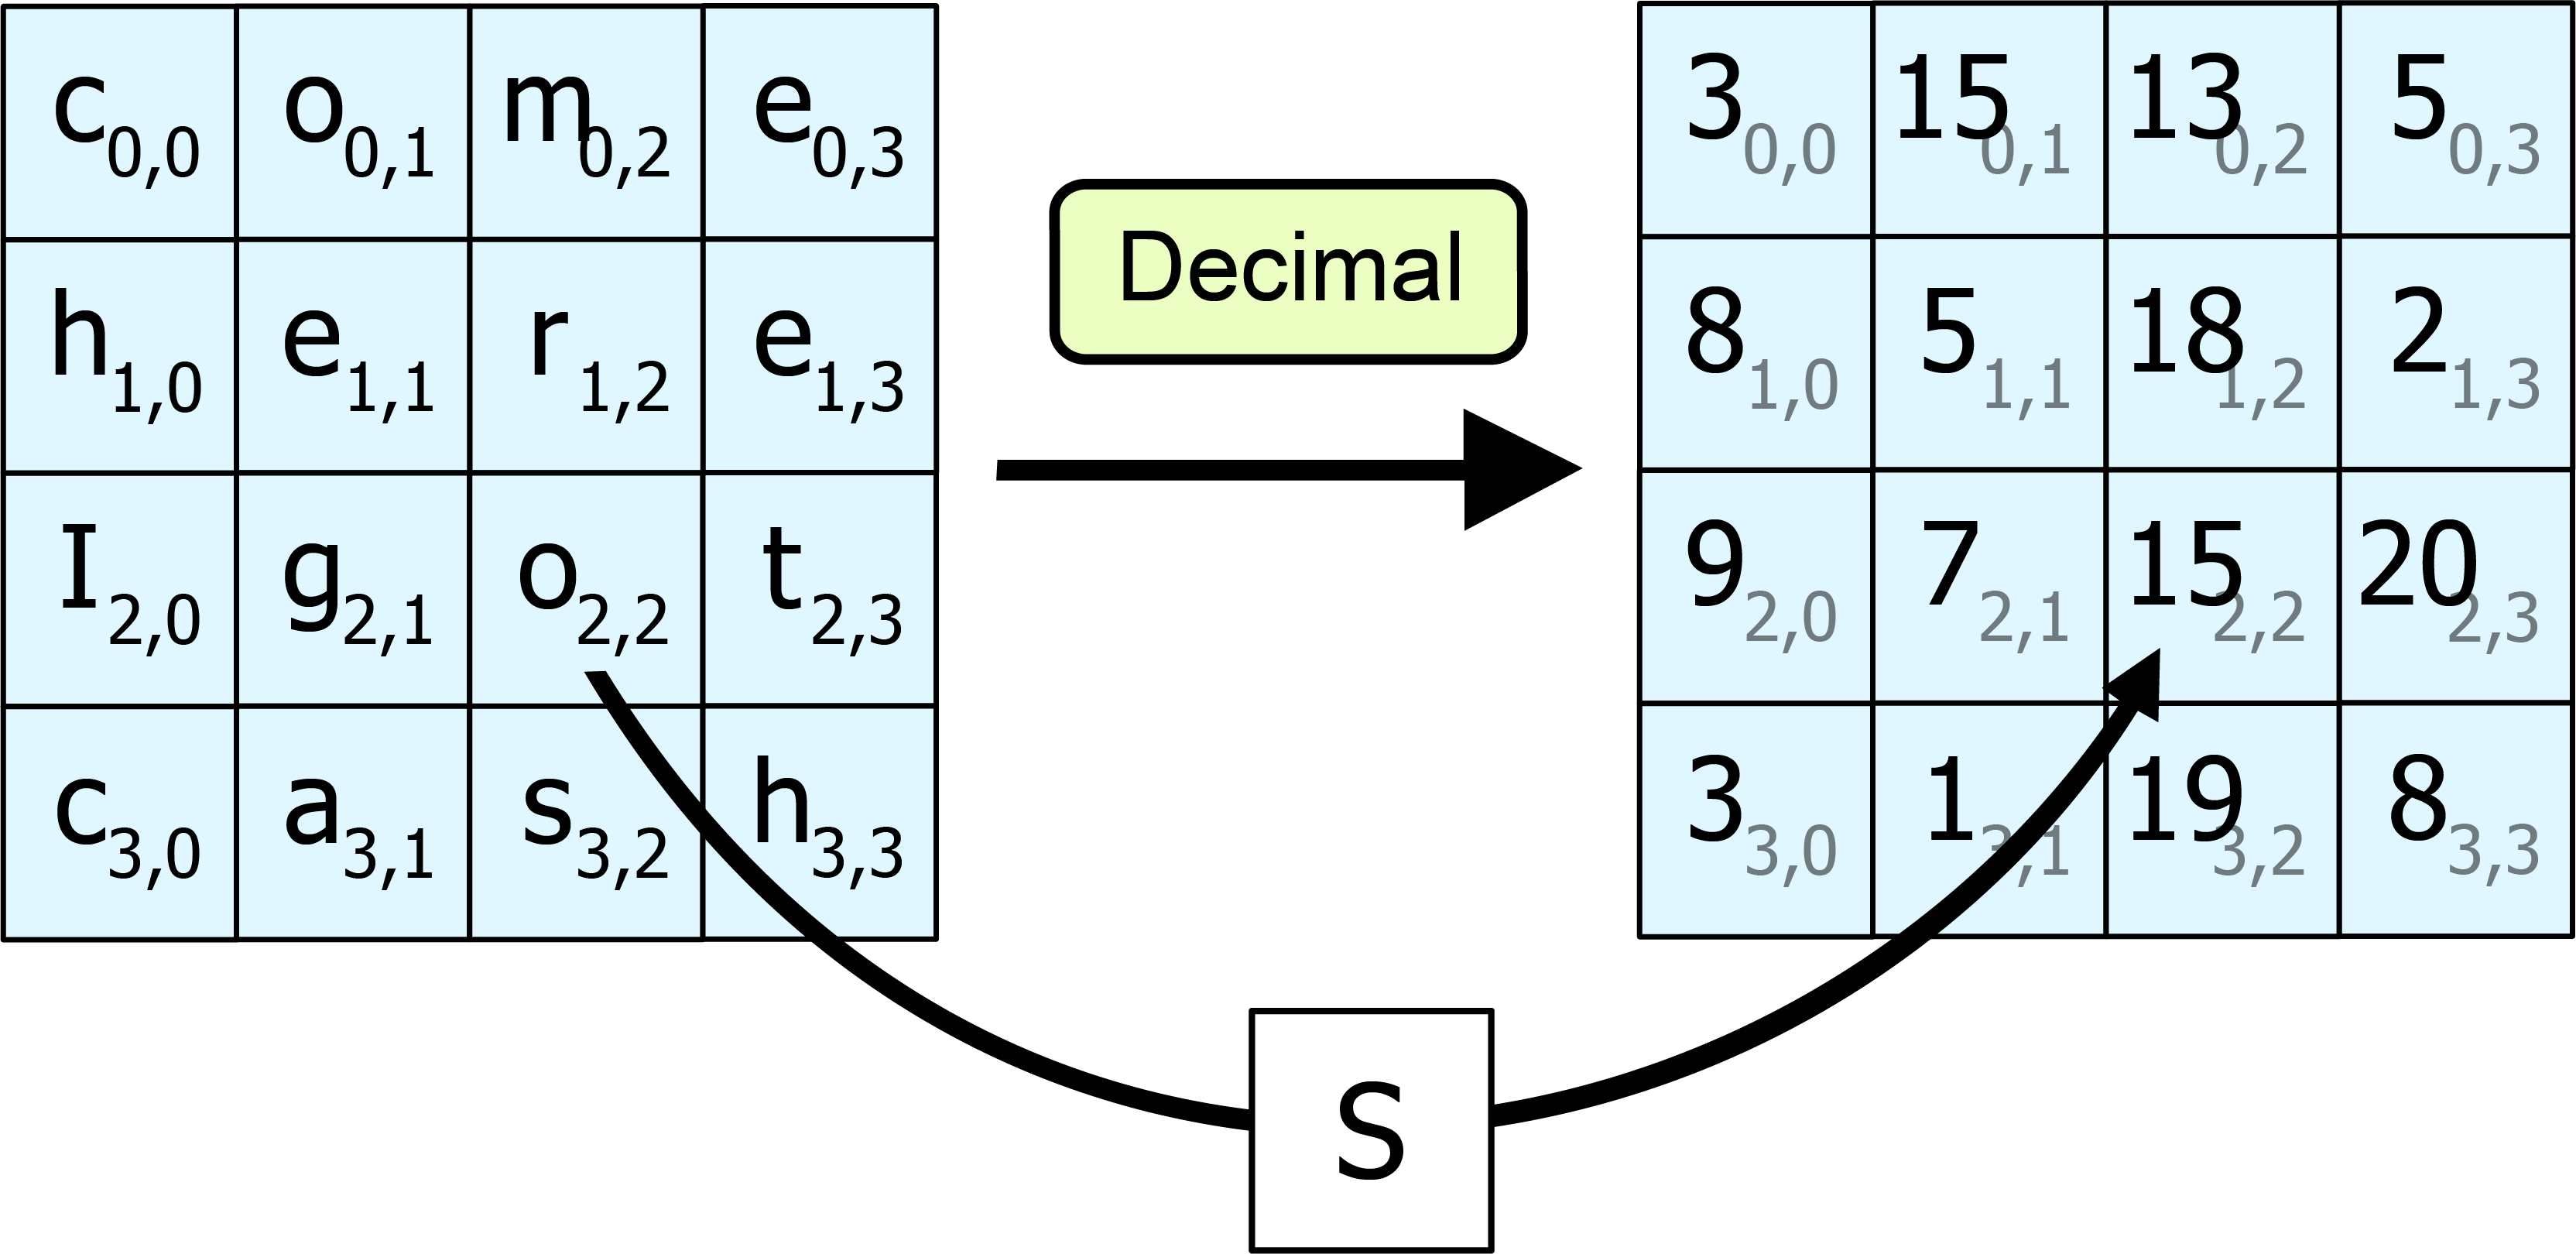
\includegraphics[scale=0.275]{conversion_AES_1.png}
\center 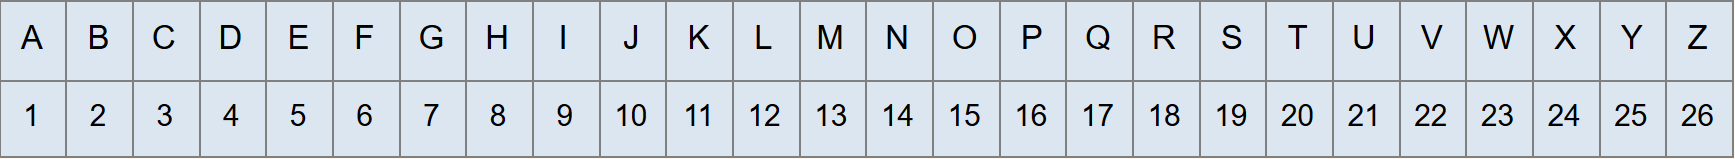
\includegraphics[scale=0.275]{numerical.png}
\end{frame}

\begin{frame}\frametitle{Shifting rows}
	\begin{enumerate}[1]
		\item First row is unchanged
		\item Second row is shifted to the left 1 time
		\item Third row is shifted to the left 2 times
		\item Fourth row is shifted to the left 3 times
	\end{enumerate}	
	\center 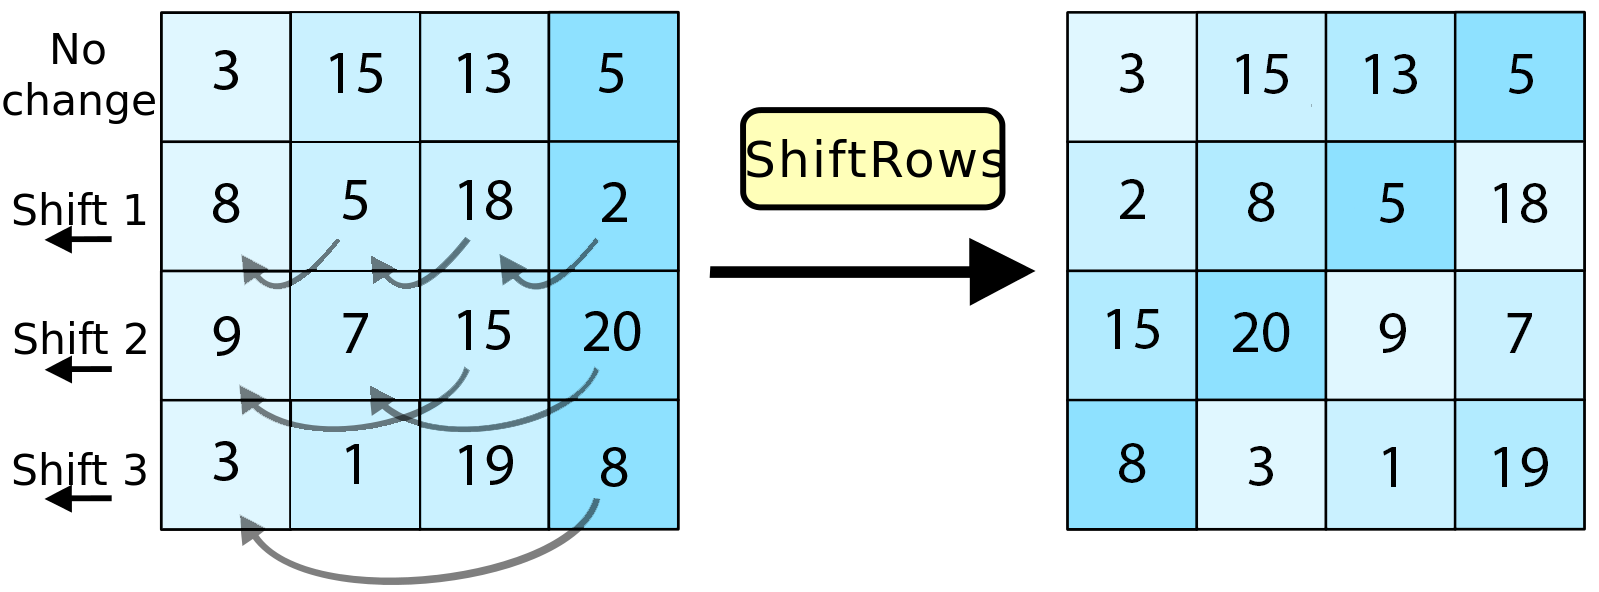
\includegraphics[scale=0.15]{shift_rows_1.png}
\end{frame}

\begin{frame}\frametitle{Mixing the columns}
	The four decimals in each column are transformed using a linear transformation
	\center In this example, we'll scale the second column by 2
	\center 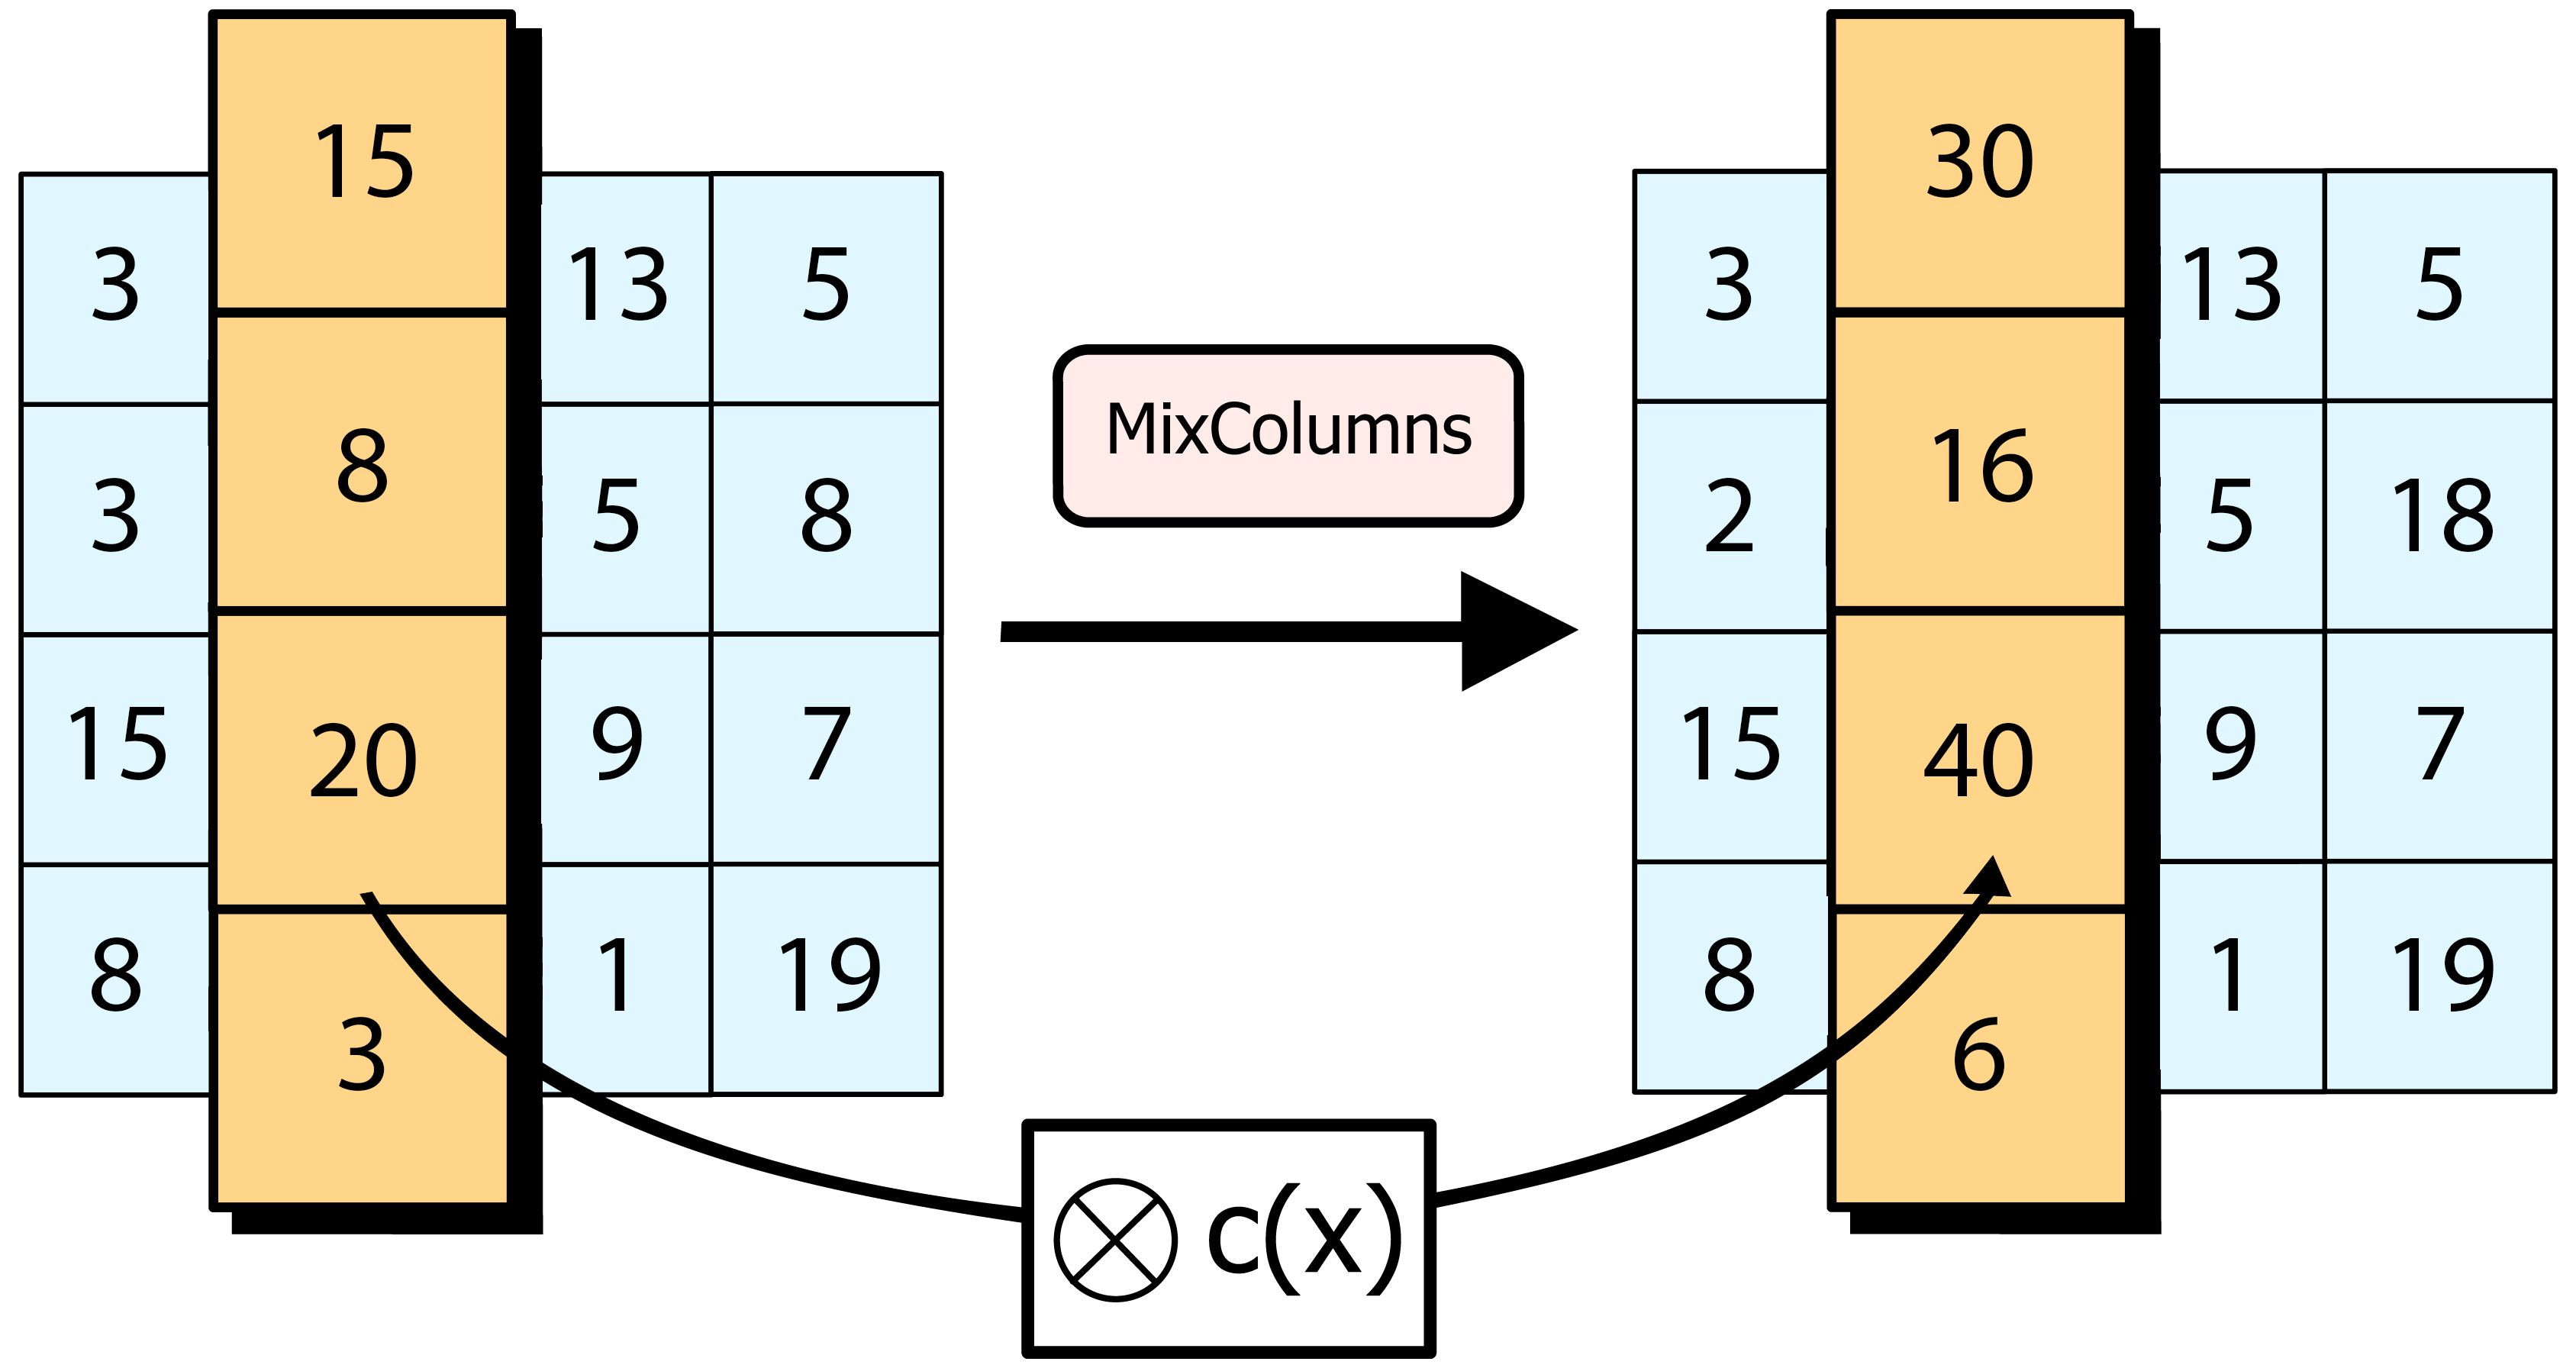
\includegraphics[scale=0.05]{mix_column_1.png}
\end{frame}

\begin{frame}\frametitle{Adding round keys}
	We then multiply the matrix by another randomly generated invertible matrix, which is the private key
	\center 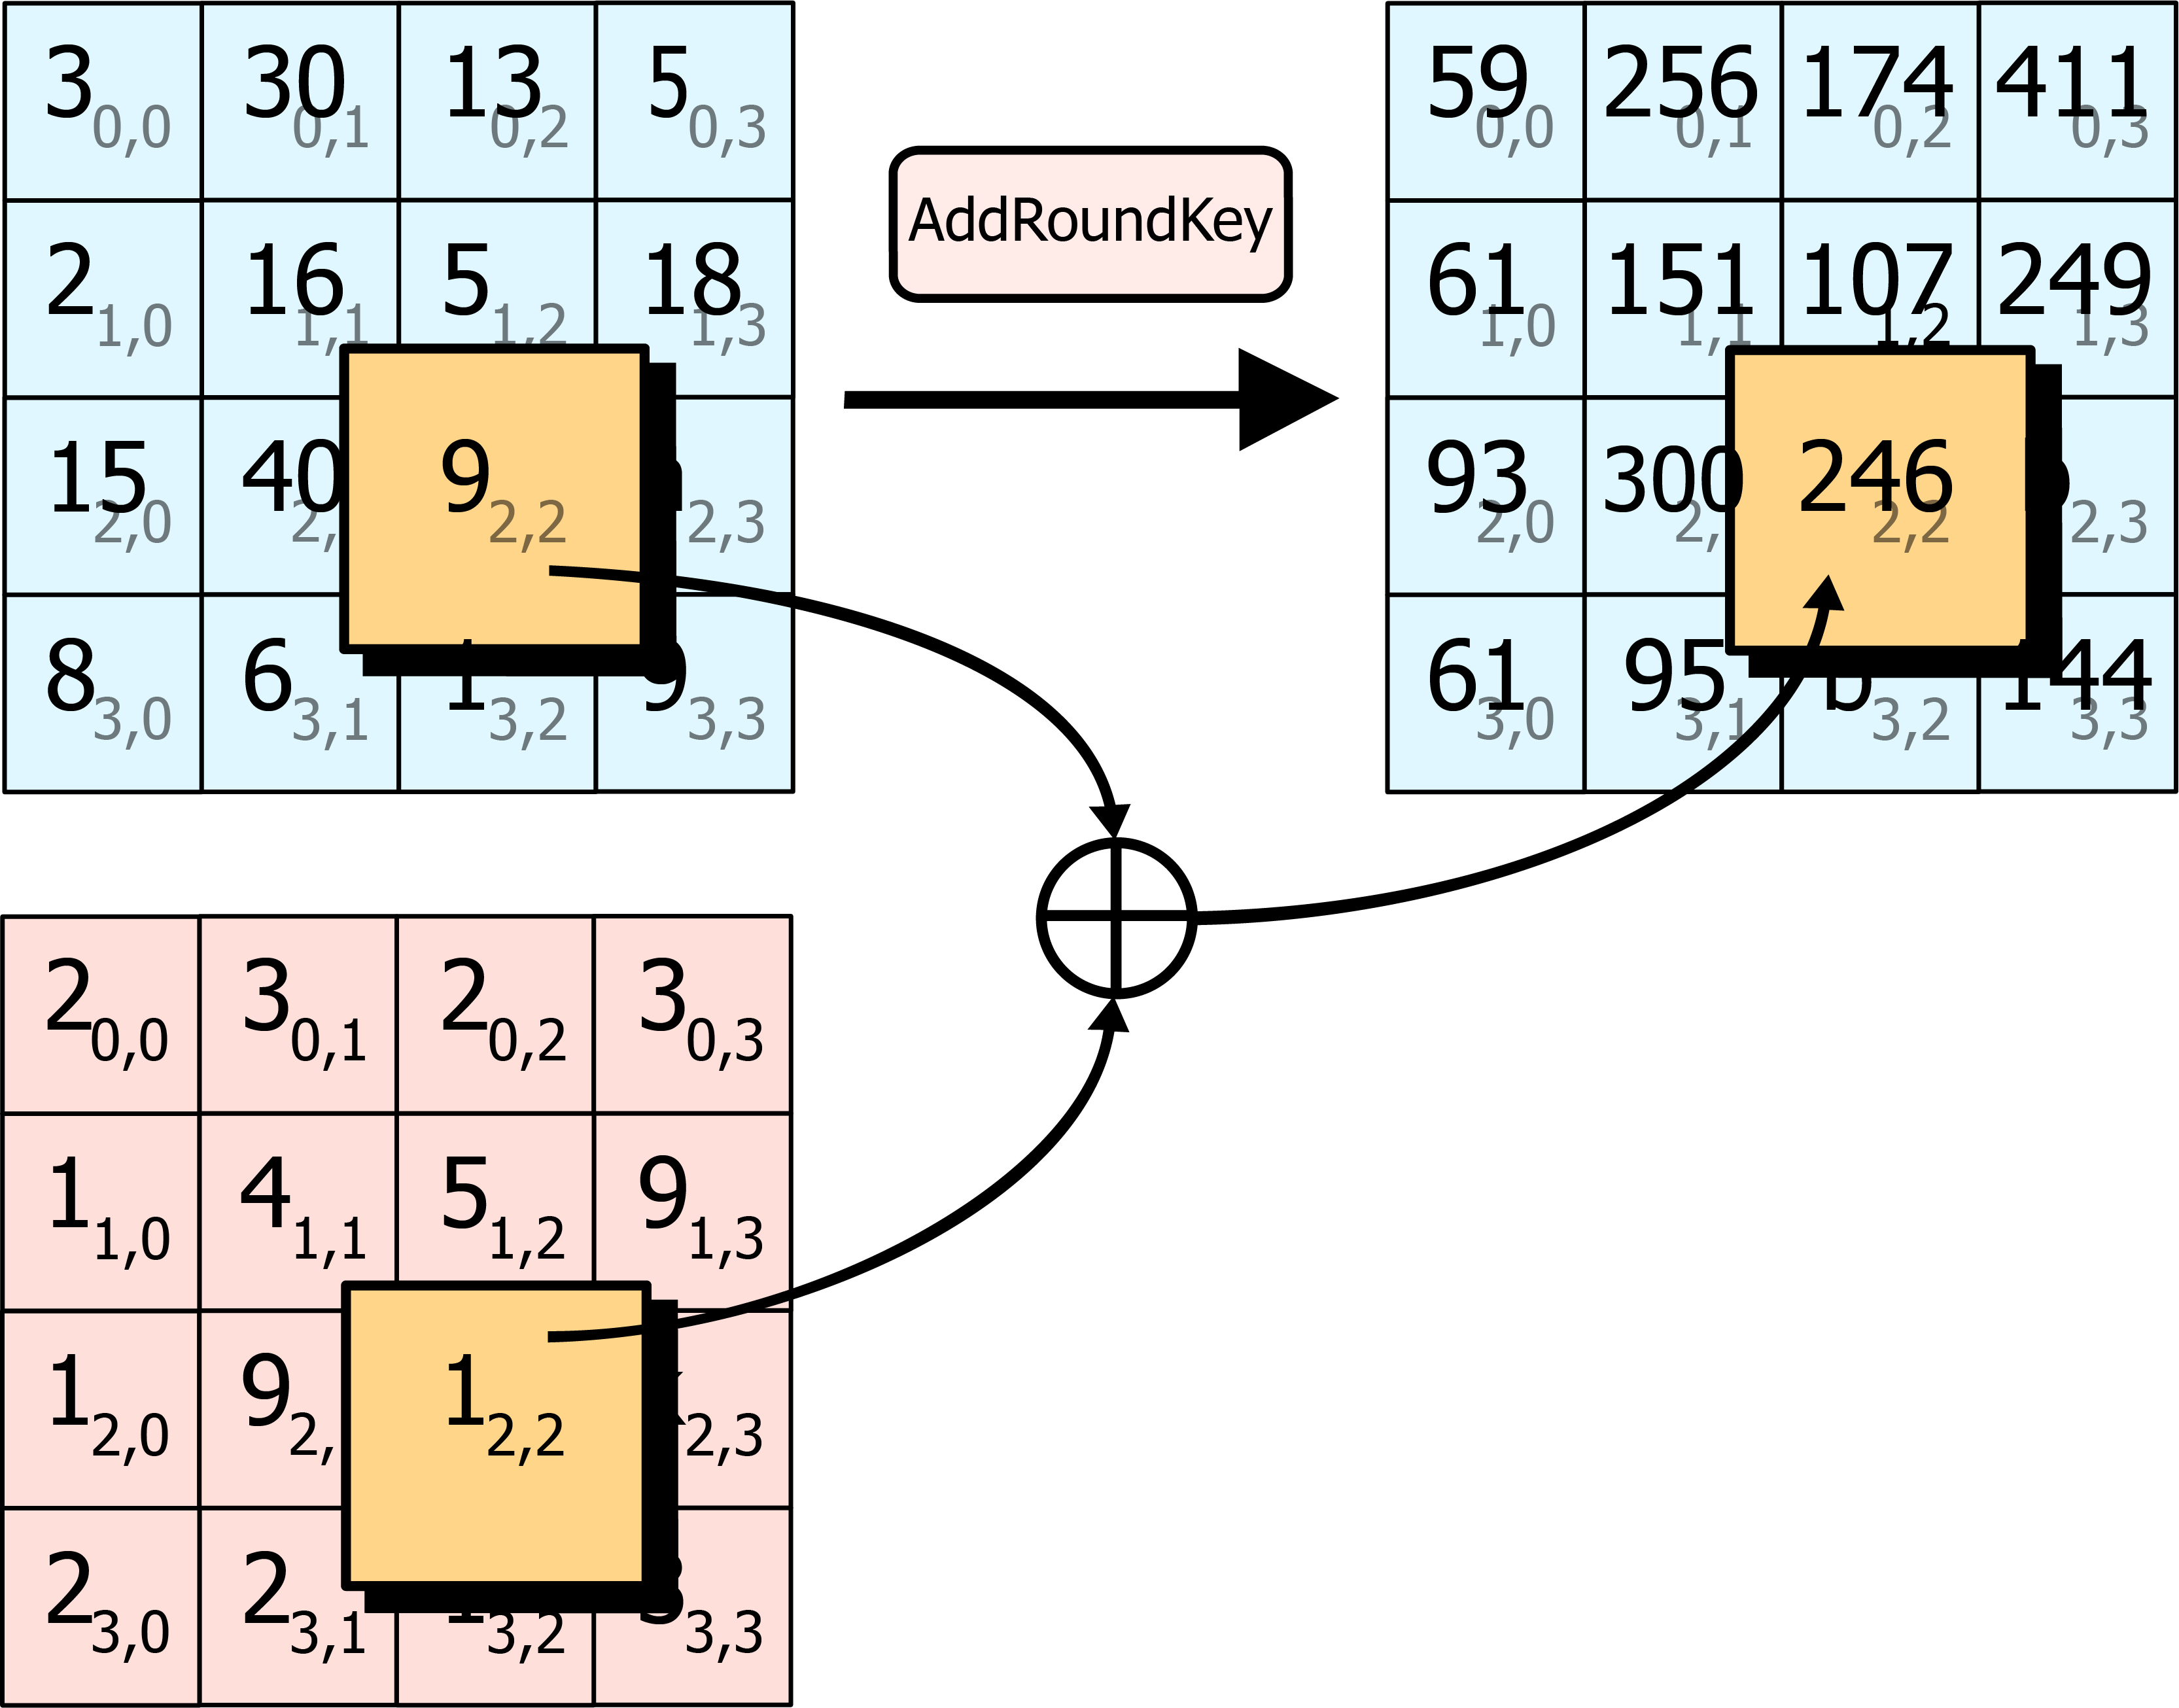
\includegraphics[scale=0.25]{add_round_key.png}
\end{frame}

\begin{frame}\frametitle{Sending and Deciphering}
	After encrypting the matrix, it is now secure to be sent to the recipient(s).\\
	To decrypting, we can decipher the message using the private key that contains all the operation backward!
\end{frame}

\section{Conclusion}
\begin{frame}\frametitle{Conclusion}
	\begin{enumerate}[]
	\item Encryption plays an essential role in securing our private data.
	\item The examples use Linear Algebra to handle the Math, but there can be other methods!
	\end{enumerate}
\end{frame}

\begin{frame}
	\center Thank you very much for watching!
\end{frame}

\begin{frame}\frametitle{Reference}
References :
	$https://searchsecurity.techtarget.com/definition/Advanced-Encryption-Standard$
Resources:
	$http://people.wku.edu/david.neal/307/Unit4/Crypt.pdf$
	$http://web.csulb.edu/~jchang9/m247/m247_fa11_David_Diego_Alissa_Daniel.pdf$

\end{frame}

\end{document}